\documentclass[tikz, crop, border = {2pt 2pt 2pt 2pt}]{standalone}

\usepackage{physics}
\usetikzlibrary{decorations.pathreplacing, calligraphy}
\usetikzlibrary{calc}

\usepackage{concmath-otf}

\begin{document}
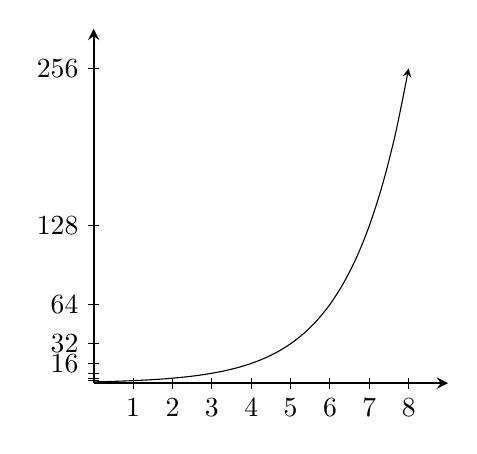
\begin{tikzpicture}
    \draw[thick, -stealth] (0, 0) -- (4.5, 0);
    \draw[thick, -stealth] (0, 0) -- (0, 4.5);

    \foreach \x in {1, 2,..., 8} {
        \draw (\x/2, 2pt) -- ++ (0, -4pt) node[below]{$\x$};
    }
    \foreach \x in {1, 2,..., 8} {
        \draw (2pt, {2^\x/64}) -- ++ (-4pt, 0);
    }
    \foreach \x in {4, 5, 6, 7, 8} {
        \pgfmathsetmacro{\y}{2^\x}
        \node[left] at (-2pt, {2^\x/64}){\pgfmathprintnumber[precision=0]{\y}};
    }
    \draw[smooth, domain = 0:8, -stealth] plot (\x/2, {2^\x/64});
\end{tikzpicture}
\end{document}